\documentclass[../../main.tex]{subfiles}

\graphicspath{{../../image/}{../../figure/}}

\begin{document}

在本章中，我们将通过具体示例来讨论一些概率分布和它们的性质。这些分布除了常规的用途之外，还是构建更复杂模型的基石，因此本书将广泛使用它们。

本章所讨论的分布有一个作用，即在给定随机变量 $x$ 的有限个观测值 $x_1,\cdots,x_N$ 的情况下，对其分布 $p(x)$ 进行建模。这就是密度估计（density estimation）问题。需要强调的是，密度估计问题基本上是不适定的，因为可能存在无数个概率分布都能产生这样一组观测值。事实上，任意在 $x_1,\cdots,x_N$ 处非零的分布 $p(x)$ 都有可能是真实的概率分布。选择合适分布的问题与模型选择有关，而该问题我们已经在多项式曲线拟合这一机器学习核心问题中遇到过（参见\cref{section:ch01-一个教学示例}）。

在对连续变量的 Gauss 分布进行考察之前，首先考虑离散变量的分布。这些分布是参数分布的典型例子，之所以如此命名，是因为这些分布仅由很少的可调参数决定，如 Gauss 分布中的均值和方差等。为了将这些模型应用于密度估计问题，我们需要一种在给定观测数据集的情况下确定合适参数值的方法（主要聚焦于最大化似然函数）。

在本章中，我们假设观测数据是独立同分布的（independent and identically distributed，i.i.d.）。在后续章节中，我们还将探索包含结构化数据的更复杂情形，到那时，这一假设将不再成立。

参数化方法的一个局限在于，它将分布假设为一种特定的函数形式，而这一做法可能在特定的应用中并不合适。另一种方法是非参数（nonparametric）密度估计方法，此时分布的形式通常取决于数据集的大小。这类模型仍然包含一些参数，但这些参数控制的是模型的复杂度而不是分布的形式。在本章的最后，我们将简述 3 种典型的非参数化方法，它们分别基于直方图、最近邻和核函数。此类非参数化技术的一个主要局限在于它们涉及存储所有训练数据；换言之，参数的数量将随数据量的增大而增加，因此这些方法在面对大型数据集时会变得非常低效。神经网络拥有大量但数量固定的参数，基于神经网络的灵活分布使深度学习同时具备参数模型的高效和非参数模型的泛化性。

\section{离散变量}\label{section:ch03-离散变量}

首先考虑离散变量的简单分布，以二元变量为起点，随后扩展到多状态变量。

\subsection{Bernoulli 分布}\label{subsection:ch03-Bernoulli分布}

考虑一个二元随机变量 $x\in\{0,1\}$。例如，$x$ 可能描述的是抛掷硬币的结果，其中 $x=1$ 表示“正面”、$x=0$ 表示“反面”。如果这枚硬币有所损坏，则落地时正面朝上的概率和反面朝上的概率未必相等。

\begin{definition}[Bernoulli 分布]\label{definition:ch03-Bernoulli分布}
设 $x$ 为只取 $0$ 与 $1$ 两个值的随机变量。若 $x=1$ 的概率由参数 $\mu$ 给出，即
\begin{align}
p(x=1\mid\mu)=\mu
\label{align:ch03-Bernoulli正面概率}
\end{align}
其中 $0\leqslant\mu\leqslant1$，则 $p(x=0\mid\mu)=1-\mu$，于是 $x$ 的概率分布可以写成如下形式：
\begin{align}
\mathrm{Bern}(x\mid\mu)=\mu^{x}(1-\mu)^{1-x}.
\label{align:ch03-Bernoulli分布}
\end{align}
上式称为参数为 $\mu$ 的 Bernoulli 分布，记作 $\mathrm{Bern}(x\mid\mu)$。
\end{definition}

% SUPPLEMENT: parent=definition:ch03-Bernoulli分布; kind=motivation; location=紧随其后的 remark（重构新增）
\begin{remark}（重构新增）
引入 Bernoulli 分布的目的是为最简单的二值观测建立参数化模型：只要指定一个标量 $\mu$，就完全确定了分布，而 $\mu$ 可以从数据中估计。定义式\eqref{align:ch03-Bernoulli分布}采用“指数指示”的写法，把 $x=1$ 与 $x=0$ 两种情形压缩进同一个表达式：当 $x=1$ 时因子 $(1-\mu)^{1-x}$ 的指数为 $0$，只留下 $\mu$；当 $x=0$ 时 $\mu^{x}$ 的指数为 $0$，只留下 $1-\mu$。这种写法便于求似然、取对数并把分布改写成指数族形式（见\cref{section:ch03-指数族分布}）。

条件 $0\leqslant\mu\leqslant1$ 是分布良定义的必要条件：若 $\mu<0$ 或 $\mu>1$，则 $\mu$ 与 $1-\mu$ 中至少有一个为负，$\mu^{x}(1-\mu)^{1-x}$ 将取负值或非实数，无法作为概率。端点 $\mu=0$ 与 $\mu=1$ 对应退化分布（概率质量全部集中在一个取值上），此时 $0^{0}$ 按组合惯例取为 $1$，定义仍然自洽。注意 $\mu$ 是刻画“正面”这一取值的概率，一旦交换两个取值的标签，$\mu$ 就应替换为 $1-\mu$，这也是\cref{exercise:ch03-02}讨论对称写法的原因。
\end{remark}

\begin{proposition}[Bernoulli 分布的归一化、均值与方差]\label{proposition:ch03-Bernoulli矩}
设 $x\sim\mathrm{Bern}(x\mid\mu)$，$0\leqslant\mu\leqslant1$。则
\begin{align}
\sum_{x=0}^{1}p(x\mid\mu)=1,
\label{align:ch03-Bernoulli归一化}
\end{align}
并且 $x$ 的均值与方差分别为
\begin{align}
\mathbb{E}[x]=\mu,
\label{align:ch03-Bernoulli均值}
\end{align}
\begin{align}
\mathrm{var}[x]=\mu(1-\mu).
\label{align:ch03-Bernoulli方差}
\end{align}
\end{proposition}
\begin{proof}
（重构新增）由\eqref{align:ch03-Bernoulli分布}，$x$ 只取 $0$ 与 $1$ 两个值，且 $p(x=1\mid\mu)=\mu$、$p(x=0\mid\mu)=1-\mu$，故
\begin{align*}
\sum_{x=0}^{1}p(x\mid\mu)=p(0\mid\mu)+p(1\mid\mu)=(1-\mu)+\mu=1,
\end{align*}
即\eqref{align:ch03-Bernoulli归一化}成立。类似地，
\begin{align*}
\mathbb{E}[x]=\sum_{x=0}^{1}x\,p(x\mid\mu)=0\cdot(1-\mu)+1\cdot\mu=\mu,
\end{align*}
即\eqref{align:ch03-Bernoulli均值}成立。对于方差，先计算二阶矩：
\begin{align*}
\mathbb{E}[x^{2}]=\sum_{x=0}^{1}x^{2}p(x\mid\mu)=0^{2}\cdot(1-\mu)+1^{2}\cdot\mu=\mu,
\end{align*}
由于 $x^{2}=x$（$x$ 只取 $0,1$），于是
\begin{align*}
\mathrm{var}[x]=\mathbb{E}[x^{2}]-\mathbb{E}[x]^{2}=\mu-\mu^{2}=\mu(1-\mu),
\end{align*}
即\eqref{align:ch03-Bernoulli方差}成立。
\end{proof}

% SUPPLEMENT: parent=proposition:ch03-Bernoulli矩; kind=motivation; location=紧随其后的 remark（重构新增）
\begin{remark}（重构新增）
这三条结论刻画了 Bernoulli 分布的“全部”低阶信息：归一化说明它是一个合法的概率分布，均值为 $\mu$ 说明参数 $\mu$ 就是“$x=1$ 的概率”这一直观含义，方差 $\mu(1-\mu)$ 说明当 $\mu=1/2$ 时不确定性最大、当 $\mu\to0$ 或 $\mu\to1$ 时不确定性趋于零。

条件 $0\leqslant\mu\leqslant1$ 在证明中只用到了“$1-\mu\geqslant0$”这一事实，用以保证两项都是非负的概率；对均值和方差的计算本身在形式上并不需要该条件，但若不满足它，$\mathbb{E}[x]=\mu$ 就不再是“概率的加权平均”，方差也可能为负，失去意义。方差公式中的 $\mu(1-\mu)$ 在 $\mu\in[0,1]$ 上非负且以 $1/4$ 为最大值，这一上界在后面讨论 Bernoulli 分布的熵（\cref{exercise:ch03-01}）时还会再次出现。
\end{remark}

假设我们有一个包含 $x$ 的观测值的数据集 $\mathcal{D}=\{x_1,\cdots,x_N\}$。基于所有观测值都是独立地从 $p(x\mid\mu)$ 生成的，我们可以建立以 $\mu$ 为参数的似然方程，使得
\begin{align}
p(\mathcal{D}\mid\mu)=\prod_{n=1}^{N}p(x_n\mid\mu)=\prod_{n=1}^{N}\mu^{x_n}(1-\mu)^{1-x_n}.
\label{align:ch03-Bernoulli似然}
\end{align}

我们可以通过最大化似然方程，或等价地最大化对数似然函数（对数似然函数是单调函数）来估计 $\mu$ 的值。Bernoulli 分布的对数似然函数形式如下：
\begin{align}
\ln p(\mathcal{D}\mid\mu)=\sum_{n=1}^{N}\ln p(x_n\mid\mu)=\sum_{n=1}^{N}\bigl\{x_n\ln\mu+(1-x_n)\ln(1-\mu)\bigr\}.
\label{align:ch03-Bernoulli对数似然}
\end{align}

注意对数似然函数仅依赖 $x_n$ 的 $N$ 个观测值的和 $\sum_{n=1}^{N}x_n$。该值给出了数据在这一分布下的充分统计量（sufficient statistic）（参见\cref{section:ch03-指数族分布}）。

\begin{proposition}[Bernoulli 分布的最大似然估计]\label{proposition:ch03-Bernoulli最大似然}
设 $\mathcal{D}=\{x_1,\cdots,x_N\}$ 是来自 $\mathrm{Bern}(x\mid\mu)$ 的独立同分布观测，其中 $0<\mu<1$。则对数似然\eqref{align:ch03-Bernoulli对数似然}的唯一驻点，即 $\mu$ 的最大似然估计，为
\begin{align}
\mu_{\mathrm{ML}}=\frac{1}{N}\sum_{n=1}^{N}x_n.
\label{align:ch03-Bernoulli均值估计}
\end{align}
若记观测到 $x=1$（正面）的次数为 $m$，则\eqref{align:ch03-Bernoulli均值估计}又可写作
\begin{align}
\mu_{\mathrm{ML}}=\frac{m}{N}.
\label{align:ch03-Bernoulli比例估计}
\end{align}
\end{proposition}
\begin{proof}
（重构新增）记 $\ell(\mu)=\ln p(\mathcal{D}\mid\mu)$。由\eqref{align:ch03-Bernoulli对数似然}，
\begin{align*}
\ell(\mu)=\Bigl(\sum_{n=1}^{N}x_n\Bigr)\ln\mu+\Bigl(N-\sum_{n=1}^{N}x_n\Bigr)\ln(1-\mu),
\end{align*}
其中用到了 $\sum_{n}(1-x_n)=N-\sum_{n}x_n$。对 $\mu$ 求导得
\begin{align*}
\frac{\mathrm{d}\ell}{\mathrm{d}\mu}=\frac{1}{\mu}\sum_{n=1}^{N}x_n-\frac{1}{1-\mu}\Bigl(N-\sum_{n=1}^{N}x_n\Bigr).
\end{align*}
令导数为零，两边乘以 $\mu(1-\mu)$（在 $0<\mu<1$ 时为正），得
\begin{align*}
(1-\mu)\sum_{n=1}^{N}x_n=\mu\Bigl(N-\sum_{n=1}^{N}x_n\Bigr),
\end{align*}
即 $\sum_{n}x_n=\mu N$，故驻点唯一，且 $\mu_{\mathrm{ML}}=\frac{1}{N}\sum_{n}x_n$，这就是\eqref{align:ch03-Bernoulli均值估计}。

再验证它给出最大值。二阶导数为
\begin{align*}
\frac{\mathrm{d}^{2}\ell}{\mathrm{d}\mu^{2}}=-\frac{1}{\mu^{2}}\sum_{n=1}^{N}x_n-\frac{1}{(1-\mu)^{2}}\Bigl(N-\sum_{n=1}^{N}x_n\Bigr)<0,
\end{align*}
因为两项都非正，且当 $0<\sum_{n}x_n<N$ 时两项都严格为负。故 $\ell$ 在 $(0,1)$ 上严格凹，唯一驻点即为全局最大值点。

最后，若 $x=1$ 出现 $m$ 次，则 $\sum_{n}x_n=m$，于是 $\mu_{\mathrm{ML}}=m/N$，即\eqref{align:ch03-Bernoulli比例估计}。
\end{proof}

% SUPPLEMENT: parent=proposition:ch03-Bernoulli最大似然; kind=motivation; location=紧随其后的 remark（重构新增）
\begin{remark}（重构新增）
最大似然估计的推导说明了“对数把乘积变成求和”这一技巧为何重要：取对数后数据只通过 $\sum_n x_n$ 进入似然，这就是充分统计量的雏形（\cref{section:ch03-指数族分布}将给出一般定义）。

证明中要求 $0<\mu<1$，原因是 $\ln\mu$ 与 $\ln(1-\mu)$ 只在开区间上有定义；端点情形应直接处理：若全部观测为 $x_n=1$，则似然 $\mu^{N}$ 在 $\mu=1$ 处取最大值 $\mu_{\mathrm{ML}}=1$；若全部观测为 $x_n=0$，则 $\mu_{\mathrm{ML}}=0$。这两种退化情形下 $\mu_{\mathrm{ML}}=m/N$ 仍然成立，只是不再由求导得到。此外，若 $m=0$ 或 $m=N$，二阶导数在驻点处退化，但由 $0^{0}$ 的惯例直接代入即可验证似然在该点的取值最大。
\end{remark}

这样硬币落地时正面朝上的概率就可以在上述最大化似然的框架下，通过在数据集中计算正面朝上次数的比例得到。

\begin{definition}[样本均值]\label{definition:ch03-样本均值}
设 $x_1,\cdots,x_N$ 是一组观测值，则称
\begin{align}
\bar{x}\triangleq\frac{1}{N}\sum_{n=1}^{N}x_n
\label{align:ch03-样本均值}
\end{align}
为这组观测值的样本均值（sample mean）。
\end{definition}

% SUPPLEMENT: parent=definition:ch03-样本均值; kind=motivation; location=紧随其后的 remark（重构新增）
\begin{remark}（重构新增）
样本均值是\eqref{align:ch03-Bernoulli均值估计}的一般形式，它并不依赖 Bernoulli 假设。引入这一术语是为了在后面反复使用：多元 Gauss 分布的均值最大似然解\eqref{align:ch03-Gauss均值ML}正是向量形式的样本均值，序贯估计\eqref{align:ch03-序贯更新}则给出了它的递推算法。注意样本均值只对“可以相加”的量有意义，因此它适用于实值观测，而不直接适用于周期变量——这正是\cref{section:ch03-周期变量}要另行定义“圆周均值”的原因。
\end{remark}

\subsection{二项分布}\label{subsection:ch03-二项分布}

我们同样可以给出在包含 $N$ 个观测值的数据集中，有 $m$ 个观测值为 $x=1$ 的二元变量 $x$ 的分布。这一分布称为二项（binomial）分布，由\cref{align:ch03-Bernoulli似然}可以看出，它与 $\mu^{m}(1-\mu)^{N-m}$ 成比例。为得到归一化系数，注意在抛掷硬币 $N$ 次的过程中，我们需要将所有可能掷出 $m$ 次正面朝上的情况加总起来，因此二项分布可写为如下形式：
\begin{align}
\mathrm{Bin}(m\mid N,\mu)=\binom{N}{m}\mu^{m}(1-\mu)^{N-m},
\label{align:ch03-二项分布}
\end{align}
其中
\begin{align}
\binom{N}{m}\equiv\frac{N!}{(N-m)!\,m!}
\label{align:ch03-组合数}
\end{align}
是从 $N$ 个相同物品中无放回地选择 $m$ 个物品的方法总数。

\begin{definition}[二项分布]\label{definition:ch03-二项分布}
设进行了 $N$ 次相互独立的 Bernoulli 试验，每次“成功”的概率为 $\mu$，并记 $m$ 为 $N$ 次试验中成功的次数。则 $m$ 的分布为
\begin{align*}
\mathrm{Bin}(m\mid N,\mu)=\binom{N}{m}\mu^{m}(1-\mu)^{N-m},\qquad m=0,1,\cdots,N,
\end{align*}
称为参数为 $N$ 与 $\mu$ 的二项分布，其中组合数 $\binom{N}{m}$ 由\eqref{align:ch03-组合数}给出。
\end{definition}

% SUPPLEMENT: parent=definition:ch03-二项分布; kind=motivation; location=紧随其后的 remark（重构新增）
\begin{remark}（重构新增）
二项分布回答的是“计数”的问题：把 $N$ 次独立的 Bernoulli 观测相加，就得到成功次数 $m$。这正是\cref{align:ch03-Bernoulli似然}中“数据只通过 $\sum_n x_n$ 进入似然”的另一面——当数据是 $N$ 次试验时，$\sum_n x_n$ 恰好就是 $m$，其分布自然由二项分布描述。

条件有三项：$N$ 为固定正整数、各次试验相互独立、每次试验的成功概率同为 $\mu$。$N$ 固定保证了 $m$ 的取值范围 $0\leqslant m\leqslant N$ 有限；独立性与同分布性是 $\mu^{m}(1-\mu)^{N-m}$ 这一乘积形式成立的前提，若各次试验的概率不同，则分布不再是二项分布（而是一般的 Poisson 二项分布）。组合数因子 $\binom{N}{m}$ 处理的是“顺序”：$m$ 次成功可以出现在 $N$ 个位置中的任意 $m$ 个位置上，且这些情形互斥，故概率相加。
\end{remark}

\cref{figure:ch03-二项分布直方图}展示了一个 $N=10$、$\mu=0.25$ 的二项分布（见\cref{exercise:ch03-03}）。

对于独立的事件，和的均值就是均值的和，而和的方差就是方差的和。用这些结果就能找到二项分布的均值和方差（见\cref{proposition:ch03-二项矩}的证明）。由于 $m=x_1+\cdots+x_N$ 且任意观测的均值和方差均可由\cref{align:ch03-Bernoulli均值}和\cref{align:ch03-Bernoulli方差}给出，故有
\begin{align}
\mathbb{E}[m]\equiv\sum_{m=0}^{N}m\,\mathrm{Bin}(m\mid N,\mu)=N\mu,
\label{align:ch03-二项均值}
\end{align}
\begin{align}
\mathrm{var}[m]\equiv\sum_{m=0}^{N}(m-\mathbb{E}[m])^{2}\,\mathrm{Bin}(m\mid N,\mu)=N\mu(1-\mu).
\label{align:ch03-二项方差}
\end{align}

\begin{proposition}[二项分布的均值与方差]\label{proposition:ch03-二项矩}
设 $m\sim\mathrm{Bin}(m\mid N,\mu)$，$0\leqslant\mu\leqslant1$。则
\begin{align*}
\mathbb{E}[m]=N\mu,\qquad \mathrm{var}[m]=N\mu(1-\mu).
\end{align*}
\end{proposition}
\begin{proof}
（重构新增）设 $x_1,\cdots,x_N$ 是 $N$ 次独立 Bernoulli 试验的指示变量，即 $x_n=1$ 表示第 $n$ 次成功，$x_n=0$ 表示失败，则 $m=x_1+\cdots+x_N$，且每个 $x_n$ 都服从参数为 $\mu$ 的 Bernoulli 分布。

由期望的线性性（它不要求独立性），
\begin{align*}
\mathbb{E}[m]=\sum_{n=1}^{N}\mathbb{E}[x_n]=\sum_{n=1}^{N}\mu=N\mu,
\end{align*}
其中用到\eqref{align:ch03-Bernoulli均值}。

对于方差，由独立性可知协方差为零，即 $\mathrm{cov}[x_i,x_j]=0$（$i\neq j$），于是
\begin{align*}
\mathrm{var}[m]=\sum_{n=1}^{N}\mathrm{var}[x_n]+2\sum_{i<j}\mathrm{cov}[x_i,x_j]=\sum_{n=1}^{N}\mu(1-\mu)=N\mu(1-\mu),
\end{align*}
其中用到\eqref{align:ch03-Bernoulli方差}。
\end{proof}

% SUPPLEMENT: parent=proposition:ch03-二项矩; kind=motivation; location=紧随其后的 remark（重构新增）
\begin{remark}（重构新增）
这一证明的关键是“把计数拆成指示变量之和”：一旦 $m=x_1+\cdots+x_N$，期望与方差的计算就归结为单次试验的结论。期望的线性性无需独立性，而方差的相加必须依赖独立性（严格地说是两两不相关）；若各次试验正相关，则和的方差会大于 $N\mu(1-\mu)$。

$N\mu$ 与 $N\mu(1-\mu)$ 也解释了二项分布的直观形状：当 $N$ 增大时，均值线性增长而标准差按 $\sqrt{N}$ 增长，因此相对波动 $\sqrt{\mu(1-\mu)/N}$ 越来越小，分布相对其均值越来越集中——这正是\cref{figure:ch03-二项分布直方图}以及中心极限定理所描述的现象。这些结论也可以用微积分直接对\eqref{align:ch03-二项分布}求和得到（见\cref{exercise:ch03-04}）。
\end{remark}

\begin{figure}[htbp]
  \centering
  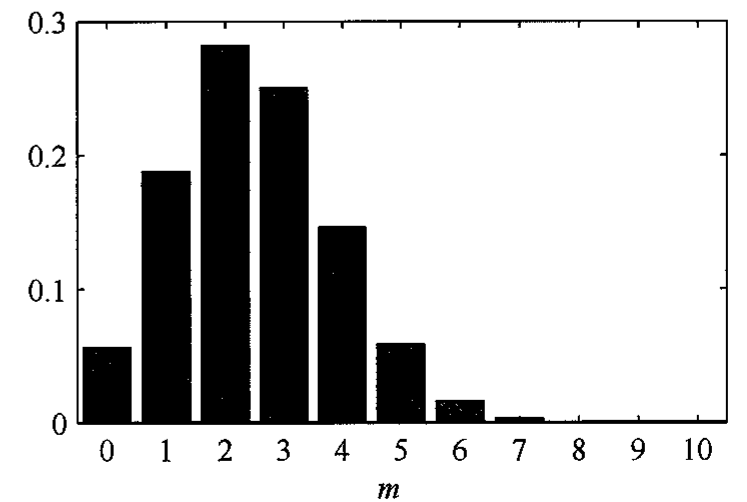
\includegraphics[width=0.62\textwidth]{ch03-fig3-1-binomial-hist.png}
  \caption{当 $N=10$ 且 $\mu=0.25$ 时，二项分布\eqref{align:ch03-二项分布}作为 $m$ 的函数的直方图。}
  \label{figure:ch03-二项分布直方图}
\end{figure}

\subsection{多项分布}\label{subsection:ch03-多项分布}

二元变量可以用于描述只有两种可能取值的量。然而通常情况下，我们遇到的离散变量可能包含 $K$ 个相互无关的状态。尽管存在多种表示这些变量的方法，但我们很快将会看到一种非常便捷的“$K$ 中之一”（1-of-$K$）的表示方案，有时又称“独热编码”。

\begin{definition}[1-of-$K$ 表示与独热编码]\label{definition:ch03-独热编码}
设离散变量有 $K$ 个互不相同的状态。称 $K$ 维向量 $\boldsymbol{x}=(x_1,\cdots,x_K)^{\mathsf{T}}$ 为该变量的 1-of-$K$ 表示或独热编码（one-hot encoding），如果 $x_1,\cdots,x_K$ 中有且仅有一个取值为 $1$，其余全部取值为 $0$，即 $\sum_{k=1}^{K}x_k=1$ 且 $x_k\in\{0,1\}$。
\end{definition}

% SUPPLEMENT: parent=definition:ch03-独热编码; kind=motivation; location=紧随其后的 remark（重构新增）
\begin{remark}（重构新增）
引入 1-of-$K$ 表示是为了把“取哪一个状态”这种类别信息写成向量，从而使概率、求和、线性代数运算都能直接施加于它。例如，若变量存在 $K=6$ 种状态，且某次观测刚好对应状态 $x_3=1$，则
\begin{align}
\boldsymbol{x}=(0,0,1,0,0,0)^{\mathsf{T}}.
\label{align:ch03-独热编码}
\end{align}
这样一来，“第 $k$ 个状态”在数值上就对应“$\boldsymbol{x}$ 的第 $k$ 个分量为 $1$”，而 $\sum_{k}x_k=1$ 恰好保证了每次观测只落在一个状态上。代价是维度随状态数线性增长：$K$ 个状态用 $K$ 维向量表示，其中 $K-1$ 个自由度是冗余的（\cref{section:ch03-指数族分布}会利用这一点把参数减到 $K-1$ 个）。
\end{remark}

如果我们将 $x_k=1$ 的概率记为 $\mu_k$，则 $\boldsymbol{x}$ 的分布可以由下式给出：
\begin{align}
p(\boldsymbol{x}\mid\boldsymbol{\mu})=\prod_{k=1}^{K}\mu_k^{x_k},
\label{align:ch03-类别分布}
\end{align}
其中 $\boldsymbol{\mu}=(\mu_1,\cdots,\mu_K)^{\mathsf{T}}$，且因为参数 $\mu_k$ 表示的是概率，它们满足约束 $\mu_k\geqslant0$ 和 $\sum_{k=1}^{K}\mu_k=1$。

\begin{definition}[类别分布]\label{definition:ch03-类别分布}
设 $\boldsymbol{x}$ 为具有 $K$ 个状态的离散变量的 1-of-$K$ 表示，参数向量 $\boldsymbol{\mu}=(\mu_1,\cdots,\mu_K)^{\mathsf{T}}$ 满足 $\mu_k\geqslant0$ 与 $\sum_{k=1}^{K}\mu_k=1$，则称
\begin{align*}
p(\boldsymbol{x}\mid\boldsymbol{\mu})=\prod_{k=1}^{K}\mu_k^{x_k}
\end{align*}
为参数为 $\boldsymbol{\mu}$ 的类别分布（categorical distribution）。
\end{definition}

% SUPPLEMENT: parent=definition:ch03-类别分布; kind=motivation; location=紧随其后的 remark（重构新增）
\begin{remark}（重构新增）
类别分布是 Bernoulli 分布在 $K>2$ 时的直接推广：把\eqref{align:ch03-Bernoulli分布}中的 $\mu^{x}(1-\mu)^{1-x}$ 换成 $\prod_k\mu_k^{x_k}$，就把“一次试验的两个结果”扩展为“一次试验的 $K$ 个结果”。由于 $\boldsymbol{x}$ 是独热向量，乘积中只有第 $k$ 个因子（对应 $x_k=1$）存活下来，其值为 $\mu_k$，其余因子都是 $\mu_j^{0}=1$。

参数空间的约束 $\mu_k\geqslant0$ 与 $\sum_k\mu_k=1$ 缺一不可：前者保证非负性，后者保证总概率为 $1$。注意这 $K$ 个参数只有 $K-1$ 个自由度，这一约束在作最大似然估计时必须用 Lagrange 乘子处理（见\cref{proposition:ch03-多项最大似然}），也是后面把它写成指数族时只保留 $M-1$ 个自然参数的原因。
\end{remark}

\cref{align:ch03-类别分布}所示的分布可以看作将 Bernoulli 分布扩展到可以描述超过两种状态。可以看出，这一分布是归一化的：
\begin{align}
\sum_{\boldsymbol{x}}p(\boldsymbol{x}\mid\boldsymbol{\mu})=\sum_{k=1}^{K}\mu_k=1,
\label{align:ch03-类别分布归一}
\end{align}
且
\begin{align}
\mathbb{E}[\boldsymbol{x}\mid\boldsymbol{\mu}]=\sum_{\boldsymbol{x}}p(\boldsymbol{x}\mid\boldsymbol{\mu})\,\boldsymbol{x}=\boldsymbol{\mu}.
\label{align:ch03-类别分布均值}
\end{align}

\begin{proposition}[类别分布的归一化与均值]\label{proposition:ch03-类别分布矩}
设 $p(\boldsymbol{x}\mid\boldsymbol{\mu})=\prod_{k=1}^{K}\mu_k^{x_k}$ 为类别分布，$\mu_k\geqslant0$，$\sum_{k=1}^{K}\mu_k=1$。则
\begin{align*}
\sum_{\boldsymbol{x}}p(\boldsymbol{x}\mid\boldsymbol{\mu})=1,\qquad \mathbb{E}[\boldsymbol{x}\mid\boldsymbol{\mu}]=\boldsymbol{\mu}.
\end{align*}
\end{proposition}
\begin{proof}
（重构新增）对 $\boldsymbol{x}$ 求和是在全部 $K$ 个可能的独热向量上进行的。由于每个独热向量恰好对应一个状态 $k$，且在该向量处 $p(\boldsymbol{x}\mid\boldsymbol{\mu})=\mu_k$，故
\begin{align*}
\sum_{\boldsymbol{x}}p(\boldsymbol{x}\mid\boldsymbol{\mu})=\sum_{k=1}^{K}\mu_k=1,
\end{align*}
这就是\eqref{align:ch03-类别分布归一}。

对于均值，由定义
\begin{align*}
\mathbb{E}[\boldsymbol{x}\mid\boldsymbol{\mu}]=\sum_{k=1}^{K}\mu_k\,\boldsymbol{e}_k,
\end{align*}
其中 $\boldsymbol{e}_k$ 是第 $k$ 个分量为 $1$、其余为 $0$ 的独热向量。上式第 $j$ 个分量为 $\sum_k\mu_k\delta_{jk}=\mu_j$，故整个向量等于 $\boldsymbol{\mu}$，即\eqref{align:ch03-类别分布均值}。
\end{proof}

% SUPPLEMENT: parent=proposition:ch03-类别分布矩; kind=motivation; location=紧随其后的 remark（重构新增）
\begin{remark}（重构新增）
这两条结论说明类别分布的参数 $\boldsymbol{\mu}$ 有明确的概率解释：它既是各状态的概率，又是独热向量的期望。归一化把 $K$ 个参数约束在一个单纯形上，这解释了为什么 $K=2$ 时只剩一个自由参数 $\mu$，与 Bernoulli 分布一致。

证明中“对 $\boldsymbol{x}$ 求和等于对状态 $k$ 求和”这一步依赖于 $\boldsymbol{x}$ 的取值集合恰好是 $K$ 个独热向量，即依赖于 1-of-$K$ 表示；若改用 $x\in\{1,\cdots,K\}$ 的标量表示，同一结论也成立，只是求和的书写方式不同。
\end{remark}

考虑包括 $N$ 个独立观测值 $\boldsymbol{x}_1,\cdots,\boldsymbol{x}_N$ 的数据集 $\mathcal{D}$。相应的似然函数有如下形式：
\begin{align}
p(\mathcal{D}\mid\boldsymbol{\mu})=\prod_{n=1}^{N}\prod_{k=1}^{K}\mu_k^{x_{nk}}=\prod_{k=1}^{K}\mu_k^{\left(\sum_{n}x_{nk}\right)}=\prod_{k=1}^{K}\mu_k^{m_k},
\label{align:ch03-类别似然}
\end{align}
从中可以看出，包含 $N$ 个数据点的似然函数其实可以只通过 $K$ 个量来定义：
\begin{align}
m_k=\sum_{n=1}^{N}x_{nk},
\label{align:ch03-充分统计量}
\end{align}
它表示观测值 $x_k=1$ 的数量，称为分布的充分统计量（sufficient statistic）（参见\cref{section:ch03-指数族分布}）。注意变量 $m_k$ 满足如下约束：
\begin{align}
\sum_{k=1}^{K}m_k=N.
\label{align:ch03-多项计数约束}
\end{align}

为找到 $\boldsymbol{\mu}$ 的最大似然解，我们需要在\eqref{align:ch03-类别分布归一}的约束下（也就是让 $\mu_k$ 的和为 $1$），关于 $\mu_k$ 最大化 $\ln p(\mathcal{D}\mid\boldsymbol{\mu})$（Lagrange 乘子法的推导参见附录）。这可以通过使用 Lagrange 乘子 $\lambda$ 并最大化
\begin{align}
\sum_{k=1}^{K}m_k\ln\mu_k+\lambda\Bigl(\sum_{k=1}^{K}\mu_k-1\Bigr)
\label{align:ch03-多项Lagrange}
\end{align}
来实现求解。令\eqref{align:ch03-多项Lagrange}关于 $\mu_k$ 的导数为零，可得
\begin{align}
\mu_k=-m_k/\lambda.
\label{align:ch03-多项驻点}
\end{align}
将\eqref{align:ch03-多项驻点}代入约束 $\sum_k\mu_k=1$ 来求 Lagrange 乘子 $\lambda$。由此可得 $\mu_k$ 的最大似然解为
\begin{align}
\mu_k^{\mathrm{ML}}=\frac{m_k}{N},
\label{align:ch03-多项ML}
\end{align}
它实际上是 $N$ 个观测值中 $x_k=1$ 的观测值所占的比例。

\begin{proposition}[类别分布的最大似然估计]\label{proposition:ch03-多项最大似然}
设 $\mathcal{D}=\{\boldsymbol{x}_1,\cdots,\boldsymbol{x}_N\}$ 是来自类别分布的独立同分布观测，$m_k=\sum_{n}x_{nk}$，$\sum_k m_k=N$，且各 $m_k>0$。则在对 $\mu_k\geqslant0$、$\sum_k\mu_k=1$ 的约束下，对数似然 $\ln p(\mathcal{D}\mid\boldsymbol{\mu})=\sum_k m_k\ln\mu_k$ 的最大值点唯一，且由\eqref{align:ch03-多项ML}给出。
\end{proposition}
\begin{proof}
（重构新增）由于 $\sum_k\mu_k=1$，可把约束吸收进目标函数，构造 Lagrange 函数
\begin{align*}
L(\boldsymbol{\mu},\lambda)=\sum_{k=1}^{K}m_k\ln\mu_k+\lambda\Bigl(\sum_{k=1}^{K}\mu_k-1\Bigr),
\end{align*}
这就是\eqref{align:ch03-多项Lagrange}。对 $\mu_k$ 求偏导并令其为零：
\begin{align*}
\frac{\partial L}{\partial\mu_k}=\frac{m_k}{\mu_k}+\lambda=0\quad\Longrightarrow\quad\mu_k=-\frac{m_k}{\lambda},
\end{align*}
即\eqref{align:ch03-多项驻点}。代入约束 $\sum_k\mu_k=1$ 得 $-\frac{1}{\lambda}\sum_k m_k=1$，由\eqref{align:ch03-多项计数约束}有 $\sum_k m_k=N$，故 $\lambda=-N$。回代即得 $\mu_k^{\mathrm{ML}}=m_k/N$，这就是\eqref{align:ch03-多项ML}。

再证唯一性与最大值性。在单纯形 $\{\mu_k\geqslant0,\ \sum_k\mu_k=1\}$ 的内部，Hessian 为对角矩阵 $\mathrm{diag}(-m_k/\mu_k^{2})$，由于各 $m_k>0$，它负定，故 $L$ 关于 $\boldsymbol{\mu}$ 严格凹，驻点必为唯一全局最大值点。当某个 $m_k=0$ 时，目标函数不含 $\mu_k$，最大值可在 $\mu_k=0$ 处取到，此时 $\mu_k^{\mathrm{ML}}=0=m_k/N$ 仍成立。
\end{proof}

% SUPPLEMENT: parent=proposition:ch03-多项最大似然; kind=motivation; location=紧随其后的 remark（重构新增）
\begin{remark}（重构新增）
最大似然解 $\mu_k^{\mathrm{ML}}=m_k/N$ 就是“经验频率”，与 Bernoulli 情形\eqref{align:ch03-Bernoulli比例估计}完全一致，这说明参数估计在这一族分布中是“数频数”的操作。

这里必须使用 Lagrange 乘子而不能直接令梯度为零，原因是约束 $\sum_k\mu_k=1$ 使 $K$ 个参数中只有 $K-1$ 个自由；若忽略约束直接对各 $\mu_k$ 求导，得到的方程组无解（梯度条件会要求所有 $m_k=0$）。证明中用到 $m_k>0$ 来保证 $\ln\mu_k$ 可微且 Hessian 负定；若某个 $m_k=0$，最优点落在单纯形的边界上，此时严格的 KKT 条件应写成互补松弛形式，但结论不变。此外，这一估计在 $N$ 较小时会把某些 $\mu_k$ 估成 $0$，从而对其他未观测状态给出零概率，这是后面讨论先验平滑（Dirichlet 先验）的动机。
\end{remark}

已知参数向量 $\boldsymbol{\mu}$ 和观测样本总数 $N$，可以考虑量 $m_1,\cdots,m_K$ 的联合条件概率分布。由\eqref{align:ch03-类别似然}可得，这一联合条件概率分布有如下形式：
\begin{align}
\mathrm{Mult}(m_1,m_2,\cdots,m_K\mid\boldsymbol{\mu},N)=\binom{N}{m_1m_2\cdots m_K}\prod_{k=1}^{K}\mu_k^{m_k},
\label{align:ch03-多项分布}
\end{align}
这就是多项分布。归一化系数是将 $N$ 个对象分为 $K$ 组的方法数，其中每组分别有 $m_1,\cdots,m_K$ 个对象，由下式给出：
\begin{align}
\binom{N}{m_1m_2\cdots m_K}=\frac{N!}{m_1!\,m_2!\cdots m_K!}.
\label{align:ch03-多项系数}
\end{align}

\begin{definition}[多项分布]\label{definition:ch03-多项分布}
设进行了 $N$ 次相互独立的类别试验，每次试验落到第 $k$ 个状态的概率为 $\mu_k$（$k=1,\cdots,K$，$\mu_k\geqslant0$，$\sum_k\mu_k=1$），记 $m_k$ 为 $N$ 次试验中落到第 $k$ 个状态的次数，则 $(m_1,\cdots,m_K)$ 的联合分布为
\begin{align*}
\mathrm{Mult}(m_1,\cdots,m_K\mid\boldsymbol{\mu},N)=\frac{N!}{m_1!\cdots m_K!}\prod_{k=1}^{K}\mu_k^{m_k},
\end{align*}
其中 $m_k\geqslant0$ 且 $\sum_k m_k=N$。该分布称为多项（multinomial）分布，它是二项分布在 $K>2$ 个状态时的推广。
\end{definition}

% SUPPLEMENT: parent=definition:ch03-多项分布; kind=motivation; location=紧随其后的 remark（重构新增）
\begin{remark}（重构新增）
多项分布与二项分布的关系是“计数向量”与“单个计数”的关系：当 $K=2$ 时，记 $m_1=m$、$m_2=N-m$，则\eqref{align:ch03-多项分布}化为 $\frac{N!}{m!(N-m)!}\mu_1^{m}\mu_2^{N-m}$，令 $\mu_1=\mu$、$\mu_2=1-\mu$ 即回到二项分布\eqref{align:ch03-二项分布}。归一化系数\eqref{align:ch03-多项系数}是多项式系数，它把 $N$ 个可分辨的试验结果按状态分组，组内不计顺序。

条件与二项分布相同（$N$ 固定、独立、同分布），只是“成功/失败”被替换为“$K$ 个互斥状态”。$\sum_k m_k=N$ 保证了计数向量位于一个 $K-1$ 维的单纯形格点上，因此多项分布的支撑集只有 $K-1$ 个自由度。
\end{remark}

注意，包含两个状态的量可以表示为二元变量并用二项分布\eqref{align:ch03-二项分布}建模，或表示为二分之一（1-of-2）变量并用分布\eqref{align:ch03-类别分布}建模，其中令 $K=2$。

\begin{remark}（重构新增）
最后这句话澄清了三个层次的关系：Bernoulli 分布描述“一次二值试验”，二项分布描述“$N$ 次二值试验的成功次数”，而类别分布与多项分布分别是它们在 $K$ 个状态上的推广。三者的参数个数不同（$\mu$；$N,\mu$；$\boldsymbol{\mu}$；$N,\boldsymbol{\mu}$），但共享同一个“独立重复试验”的生成机制，因此后续在指数族框架下（\cref{section:ch03-指数族分布}）可以把它们统一处理。
\end{remark}

\end{document}
